\section{}
% A concentrated load P acts on a cantilever, as shown in Fig. 2. The beam is constructed of a 2024-
% T4 aluminum alloy having a yield strength σyp = 290 MPa, L = 1.5 m, t = 20 mm, c = 60 mm,
% and b = 80 mm. Based on a factor of safety n = 1.2 against initiation of yielding, calculate the
% magnitude of P for α = 30◦
% . Neglect the effect of shear in bending and assume that beam twisting
% is prevented.
A concentrated load $P$ acts on a cantilever, as shown in Fig. \ref{fig:Q2ProblemDiagram}. The beam is constructed of a 2024-
T4 aluminum alloy having a yield strength $\sigma_{yp} = 290$ MPa, $L = 1.5$ m, $t = 20$ mm, $c = 60$ mm,
and $b = 80$ mm. Based on a factor of safety $n = 1.2$ against initiation of yielding, calculate the
magnitude of $P$ for $\alpha = 30^{\circ}$. Neglect the effect of shear in bending and assume that beam twisting
is prevented.
\begin{figure}[h]
    \centering
    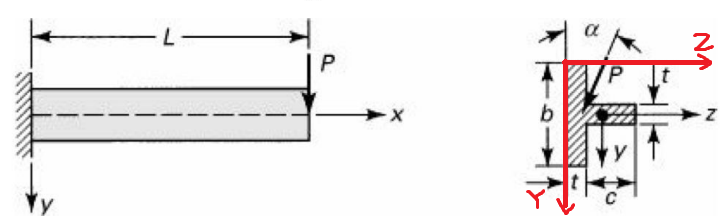
\includegraphics[width=0.35\linewidth]{Questions/Figures/Q2ProblemDiagram.png}
    \caption{Problem diagram for Question 2.}
    \label{fig:Q2ProblemDiagram}
\end{figure}

\subsection{}
First find the applied moments,
\begin{align*}
    M_y &= P_z L = -P \sin(\alpha) L  = -0.75P \\
    M_z &= P_y L = P \cos(\alpha) L = 1.30P
\end{align*}

Next, find the centroid from the reference $Z$ and $Y$ axes,
\begin{align*}
    \bar{z} = \frac{\sum \bar{z}_i A_i}{\sum A_i} = \frac{A_1 \bar{z}_1 + A_2 \bar{z}_2}{A_1 + A_2} \\
\end{align*}
where $A_1$ is the vertical rectangle and $A_2$ is the horizontal rectangle. Proceeding,
\begin{align*}
    \bar{z} &= \frac{(bt)(t/2) + (ct)(t+c/2)}{bt + ct} \\
    &= \frac{(80\times20)(20/2) + (60\times20)(20+60/2)}{80\times20 + 60\times20} \\
    &= 27.14 \text{ mm}
\end{align*}
Since the there is an axis of symmetry in the $Y$ direction, $\bar{y} = b/2 = 40$ mm.

Next, find the moments of inertia,
\begin{align*}
    I_z = \sum(I_{\bar{z}, i} + A_i d_{y, i}^2) &= I_{\bar{z}, 1} + A_1 d_{y, 1}^2 + I_{\bar{z}, 2} + A_2 d_{y, 2}^2 \\
    &= \frac{b^3t}{12} + (bt)(0)^2 + \frac{ct^3}{12} + (ct)(0)^2 \\
    &= \frac{80^3\times20}{12} + \frac{60\times20^3}{12} \\
    &= 8.93 \times 10^{5} \text{ mm}^4
\end{align*}
and
\begin{align*}
    I_y = \sum(I_{\bar{y}, i} + A_i d_{z, i}^2) &= I_{\bar{y}, 1} + A_1 d_{z, 1}^2 + I_{\bar{y}, 2} + A_2 d_{z, 2}^2 \\
    &= \frac{bt^3}{12} + (bt)(\bar{z} - t/2)^2 + \frac{c^3t}{12} + (ct)(\bar{z} - (t + c/2))^2 \\
    &= \frac{80\times20^3}{12} + (80\times20)(27.14 - 20/2)^2 + \frac{60^3\times20}{12} + (60\times20)(27.14 - (20 + 60/2))^2 \\
    &= 1.51 \times 10^{6} \text{ mm}^4
\end{align*}
Since $y$ is an axis of symmetry, $I_{yz} = 0$. Then,
\begin{align*}
    \tan{\phi} &= \frac{M_y I_z}{M_z I_y} \\
    &= \frac{-0.75P \times 8.93 \times 10^{5}}{1.30P \times 1.51 \times 10^{6}} \\
    &= -0.3412 \\ 
    \implies \phi &= \arctan(-0.3412) = \boxed{-18.84^{\circ}}
\end{align*}

\subsection{}
The maximum stress occurs at the top left corner or bottom left corner of the cross section. Using the top left corner,
\begin{align*}
    \sigma_{x} &= \frac{(M_y I_z + M_z I_{yz})z - (M_y I_{yz} + M_z I_y)y}{I_y I_z - I_{yz}^2} \\
    &= \frac{(M_y I_z \bar{z} - M_z I_y \bar{y})}{I_y I_z} \\
    &= \frac{(-0.75P \times 8.93 \times 10^{5} \times (-27.14) - 1.30P \times 1.51 \times 10^{6} \times (-40))}{1.51 \times 10^{6} \times 8.93 \times 10^{5}} \\
    &= -7.171\times 10^{-5}P
\end{align*}
By yield stress and factor of safety,
\begin{align*}
    \sigma_{x} &= \frac{-7.171 \times 10^{-5} P}{1.2} = \sigma_{yp} \\
    \implies P &= \frac{290 \times 1.2}{-7.171 \times 10^{-5}\times 10^{3}} = \boxed{-4.85 \text{ kN}}
\end{align*}